\documentclass{article}
\usepackage[english]{babel}
\usepackage[utf8x]{inputenc}
\usepackage{graphicx}
\usepackage{algorithm}
\usepackage{algorithm2e}
\usepackage{hyperref}
\usepackage{float}
%  Include course name, semester, assignment title, your name and student number. 
\title{CMPE321 - 2021 Spring \\ Project 4: Project HALO}
\date{\today}
\author{Alper Canberk Balcı, Hatice Şule Erkul, Sabri Gökberk Yılmaz \\ 2017400087, 2017400051, 2017400144}
\begin{document}
\maketitle
\newpage
\tableofcontents
\newpage
\section{Introduction}
\label{sec:introduction}
HALO, Highly Attributed
Logical Object is a digital storage management system that we found on the planet which has lost its database management system. We need to design and implement the HALO software. Halo Software is a program to manage different species living in the planet E226 − S187. You can create species, list or delete them. You can create individuals, list, search for, update or delete them.
\section{Assumptions \& Constraints}
\label{sec:ass-and-const}
Clearly specify your assumptions and constraints of the system in an itemized or tabular format. 
\subsection{Assumptions}
\begin{itemize}
    \item All fields shall be alphanumeric. Also, type and field names shall be alphanumeric.
    \item User always enters valid input. There will be no non-alphanumeric character inside the test cases.
    \item The hardware of HALO center and HALO instances will be built according to the blueprints, thus you
do not need to consider the HALO physical storage controller to interact with the storage units.
    
\end{itemize}
\subsection{Constraints}
\begin{enumerate}
    \item The data must be organized in pages and pages must contain records. So, you must clearly explain your
page and record structure in your report.
    \item You are not allowed to store all pages in the
same file and a file must contain multiple pages. This means that your system must be able to create new files as HALO grows. Moreover, when a file becomes free
due to deletions, that file must be deleted.
    \item Although a file contains multiple pages, it must
read page by page when it is needed. Loading the whole
file to RAM is not allowed.
    \item The first attribute of all types in HALO software
must be a string type, named as "planet" and its value
for all records must be "E226 − S187".
    \item The primary key of a record should be assumed to
be the value of the second field of that record.
    \item Records in the files should be stored in
descending order according to their primary keys
     
\end{enumerate}

\section{Storage Structures}
\label{sec:structures}
Explain your system catalogue, page design, page header, record header etc. with tables/diagrams/figures. 

To generate tables automatically: \url{https://www.tablesgenerator.com/}
\begin{enumerate}
    \item System Catalogue: We have an attribute catalogue 
    Attr-cat(attr-name, rel-name, type, position)
    \item File, page design: \\
    2.1. We used fixed length records, packed (white space at the end) pages. \\We don't have record headers, because we could use only primary key as record header, but it is not necessary as we retrieve primary key by taking substring of record line. \\
    Every page starts with 10 empty records for our algorithm to work. Every record starts with 12 empty fields. There is newline at the end of every record. 20*12+2=242 bytes for every line of a page. \\
    Records are stored in descending order according to their primary keys.\\ \\
    2.2. We have a page header on top of every pages of every files. Our page header consists of number of records, page id, max-primary-key, min-primary-key, and new line.\\ 20*4+2=82 bytes for page header. There is new line(2 bytes) at the end of a page. \\
    82+242*10+2 = 2504 bytes for every page. \\
    Page ids start from 1. \\
    Pages are stored in ascending order according to their page ids.\\ \\
    2.3. Our file header consists of number of pages, file id, type, max-primary-key, min-primary-key, number of fields, and a new line(2 bytes). 20*6+2=122 bytes for file header. \\
    N\textsuperscript{th} file of a type is named as \texttt{type\_nameN} \\
    There can be 20 pages at most in a file. \\
    122 + 2504*20 = 50202 bytes for a file.\\
    file ids start from 1.
\end{enumerate}
\begin{table}[H]
\centering
\begin{tabular}{|l|c|c|l|c|c|}
\hline
\textbf{no-of-pages}   & \multicolumn{1}{l|}{\textbf{file-id}} & \multicolumn{1}{l|}{\textbf{type}}  & \multicolumn{1}{l|}{\textbf{max-record}} & \multicolumn{1}{l|}{\textbf{min-record}} & \multicolumn{1}{l|}{\textbf{no-of-fields}}\\ \hline
\textbf{no-of-records} & \textbf{page-id}  & \textbf{max-record}   & \textbf{min-record} &                                    \\ \hline
\textbf{planet} &  
\textbf{record n}   & 
\textbf{field-1}   &  \textbf{field-2...}                         \\ \hline
\textbf{planet} &  
\textbf{record n-1}   & 
\textbf{field-1}   &  \textbf{field-2...}                         \\ \hline                             \\ \hline
\end{tabular}

\label{tab:ex}
\caption{An example file organization, view at the top}
\end{table}

\begin{figure}[H]
    \centering
    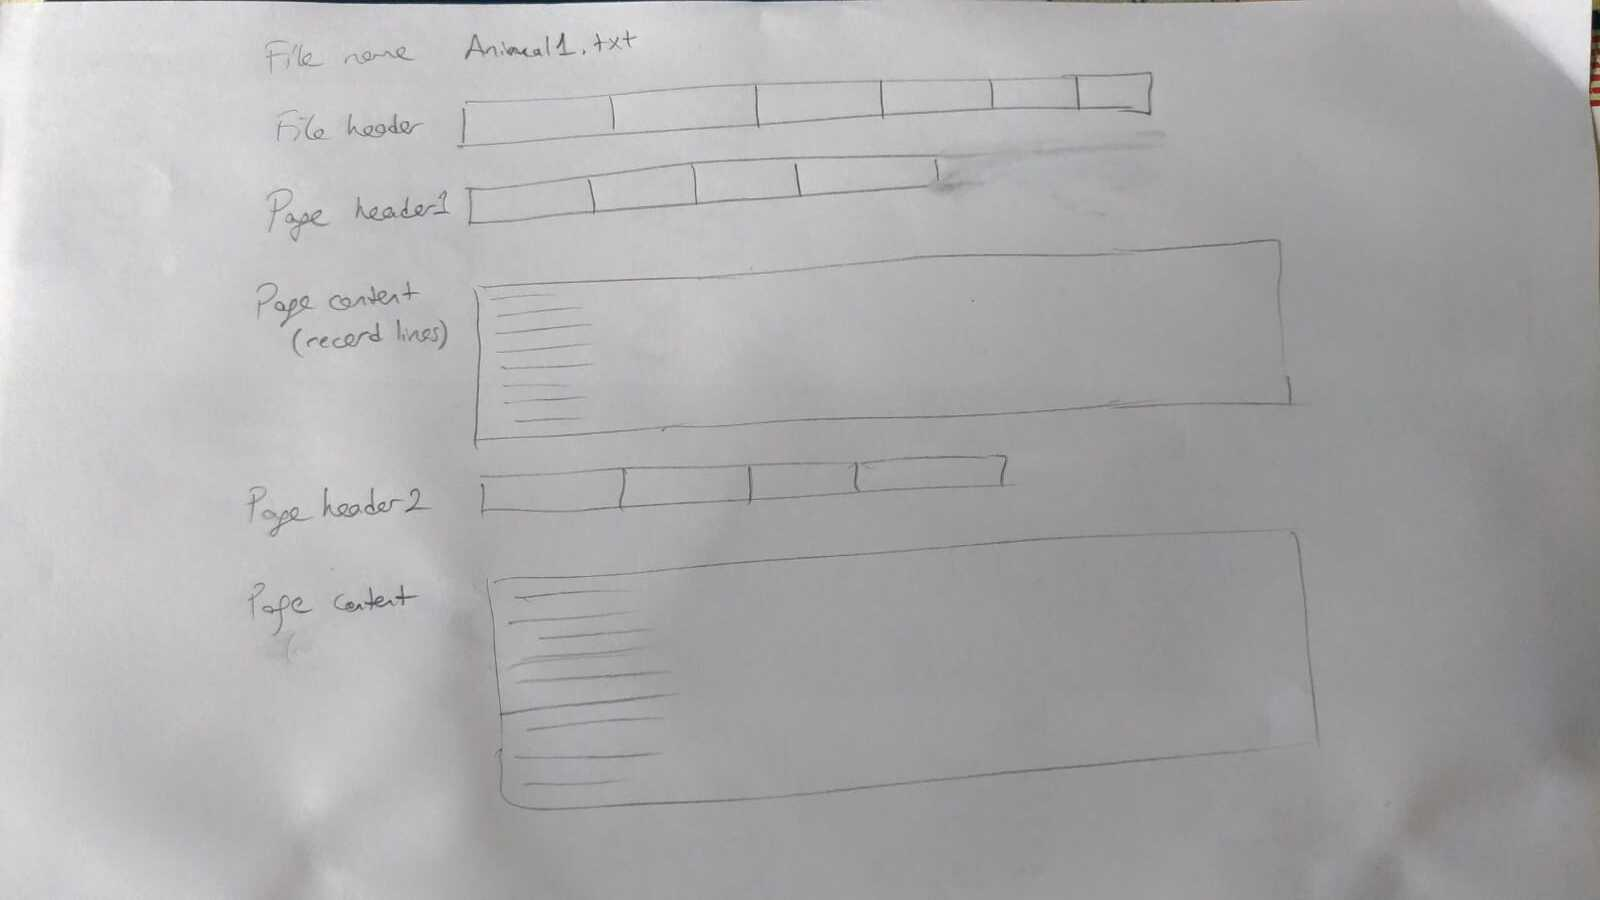
\includegraphics[width=.8\textwidth]{file-organization.jpg}
    \caption{An example figure of file organization of a file with 2 pages}
\end{figure}

\section{Operations}
\label{sec:operations}
Explaining our HALO Authentication, Definition, and Management Language Operations. Refer to the related files and functions to improve the explanation.
\subsection{HALO Authentication Language Operations}
\begin{enumerate}
    \item Login to HALO: \texttt{login\_user} function handles it. If there is already a logged in user, operation fails. It retrieves all \texttt{user\_name} password tuples from users.txt and checks if the given user-name password tuple match with any of registered users.
    \item Logout from HALO: It is handled by logout function. It sets logged-in boolean global variable to False and sets logged-user to null
    \item Register in HALO: \texttt{register\_user} function handles it, it checks if password and password repeat are the same and also if there is already a recorded account with the same \texttt{user\_name}, it returns failure. If successfully created 
\end{enumerate}
\subsection{HALO Definition Language Operations}
\begin{enumerate}
    \item Create a type:
    Creates a type, every type name is a key in \texttt{type\_file\_map} global variable and maps to list of files that belongs to the type. It calls the file object to create a file. Note that a type can have more than one files. All types have planet name and primary key as their first two columns. Rest of the fields are given as parameter. Also, a type is recorded into \texttt{type\_file\_map\_file} and \texttt{system\_catalog} whenever it is created. \texttt{create\_type} function handles these.
    \item Delete a type: When this function executes A type is deleted. Its files are deleted and it is removed from both system catalog and \texttt{type\_file\_map\_file}. \texttt{delete\_file} function does them all.
    \item Inherit a type: \texttt{inherit\_type} function does it. It looks up to system catalog and takes all fields that belong to its parent. Then, additional given fields are also included and type is created as in create type.
    \item List all types: It looks up to system catalog and displays all types that are stored in db. \texttt{list\_type} is the function that does these.
\end{enumerate}

\subsection{HALO Management Language Operations}
\begin{enumerate}
    \item Create a record: -It takes in \texttt{type\_name} and all necessary fields. \\
-Loops over file names that belong to the type.\\
-If there are no pages in a file, it creates an empty file\\
-It looks up to header of a file before reading pages. And checks to see if the record should be inserted into that file or not. If the record does not belong in that file, checks the next file.\\
-If the record belongs to that file, the code now looks for the correct page.\\
-Pages are not loaded into memory one by one and their headers are checked first. If the record belongs in the page, more actions are taken. \\
-After detecting the page id, exact location to insert the record is found by iterating over records in that file.\\
-If a file has 10 records already and the record is inserted in there, the 11\textsuperscript{th} index is removed from the file and \texttt{create\_record} is called recursively but the parameter record is the already-recorded 11\textsuperscript{th} index, since it needs a replacement and further replacements might be necessary while putting 11\textsuperscript{th} index to next page.\\
-If, the file is filled a new file is opened similar to the new page strategy.\\
-However, when we read 2502 bytes from the file, it reads 2551 bytes. We couldn’t figure out the reason behind this problem.\\
-When we insert more than 1 entry into 2\textsuperscript{nd} page, it sometimes deviates from our expected locations, hence making further insertions erroneous. :(

    
\begin{figure}[H]
\centering
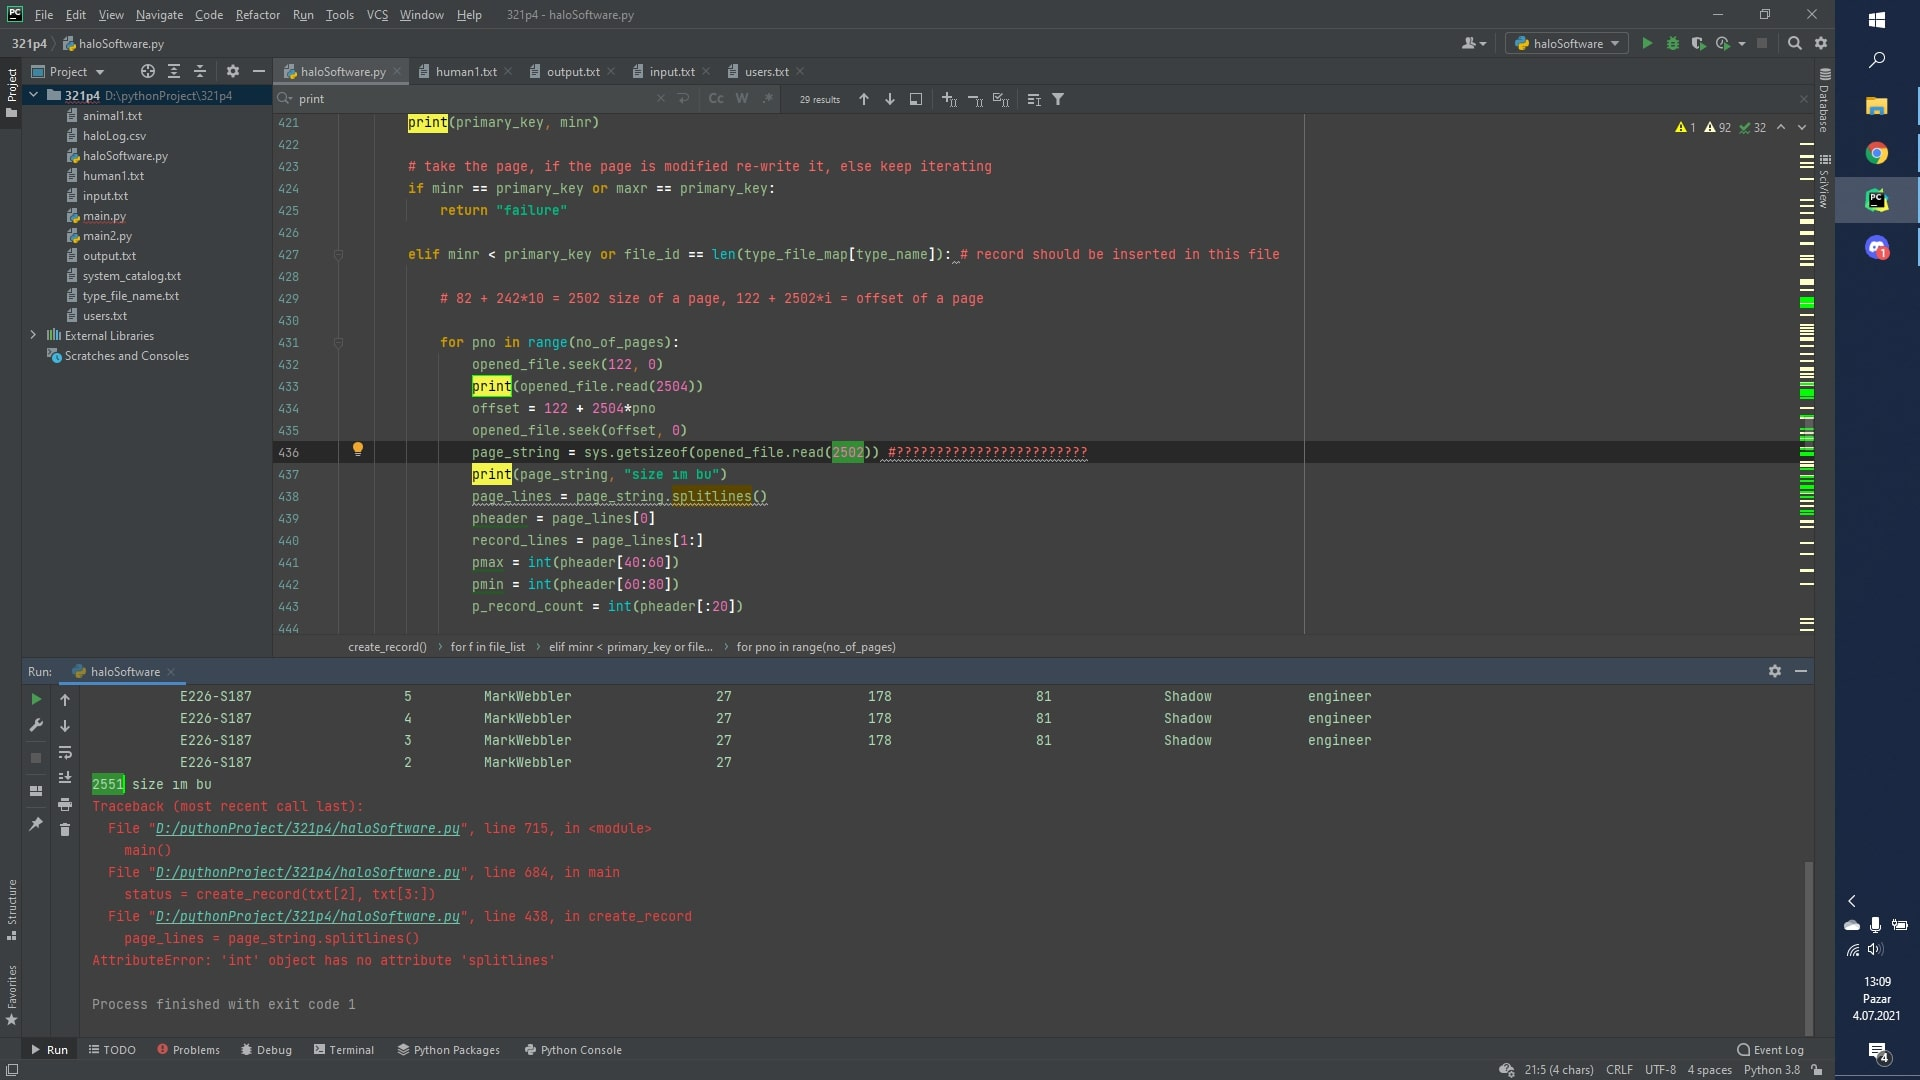
\includegraphics[width=.99\textwidth]{byte_problems.jpg}
\caption{When we want to read 2502 bytes program read 2551 bytes.}
\end{figure}

    \item Delete a record: -We get the primary key first
-We derive file names of the type name. then we traverse those files,\\
-For each file, we check file header and look up file id, number of pages It has. \\
-After that, we traverse each file with file.seek and file.read methods\\
-We get page min and page contents\\
-We iterate over all records on that page until we find the record that has the same primary key.\\
-Once the record is found we check if the page this record belongs has only one record, in this case this page can be deleted also. Same for file, if the file is empty, it can be deleted, too.\\
-If the page has more than one record we delete that record and cascade another record from the following page. \\
-We tried to cascade all entries of following pages, but it is incomplete :(

    \item Search for a record (by primary key): \texttt{search\_record} function, finds the file that it should belong through headers of files, the page that it should belong through headers of pages. If that page does not include the record, failure is returned. The record is outputted.
    \item Update a record (by primary
key): \texttt{update\_record} function, the record is searched, and if found its page is updated and written to storage. The search, read and write are all done page by page. And headers of files and pages are used in this function, too. When found, the record is updated and page is re-written. If the record not found failure is returned
    \item List all records of a type: \texttt{List\_record}: Lists all records of a given type-name. Starts with the first file and first page, iterates over pages first and files second and all records in all pages are returned.
    \item Filter records by one of the attributes of a type: Only works on primary key field and records that satisfy a given condition are returned. Headers are used for those range checks.
\end{enumerate}

\section{R \& D Discussions}
\begin{enumerate}
     \item Possible improvements: We have fixed length records causing a lot of useless empty bytes to exist.\\ We might consider making it a variable length record design to achieve efficiency in storage but there might be loss in efficiency of algorithm of management system.
     \item A HALO cluster around the LifeDome: \\
     There will be locks on the files of a type when someone tries to read or write into a file of that type to avoid interleaved execution.\\ There might be an occurrence of babies with same attributes and we might want to add them to the database at the same time. This will be a copy so system will fail one of them. \\ 
\end{enumerate}

\section{Conclusion \& Assessment}
\label{sec:conclusion}
Evaluate your design, considering its ups and downs. 
\\ Our design is very stable considering that files contains fixed length records and fixed length pages.\\ However it is not efficient in terms of storage usage because we might have excessive number of fields, excessive bytes(length) for field values. \\ In that case we should consider having more database storage units, or having an improved algorithm works on variable length records for storage.\\ \\ \\
We have problems that we pointed out in Chapter 4.3 (Create a record, Delete a record). Records cascading into an existing page(if it is not the first page) breaks the order. However, when creating a new page for the excess (11th record) record there is no problem.\\
Filter records function does not work. And we didn't call it in main function.\\
\end{document}
